\documentclass{article}

\usepackage[margin=1in]{geometry}
\usepackage{graphicx}
\usepackage{listings}
\usepackage{matlab-prettifier}
\usepackage{color}

\graphicspath{{./}}

\definecolor{gray}{rgb}{0.9,0.9,0.9}
\definecolor{mauve}{rgb}{0.58,0,0.82}
\definecolor{green}{rgb}{0,0.6,0}

\lstset{
	backgroundcolor=\color{gray},
	stepnumber=1,
	numbers=left,
	title=\lstname,
	extendedchars=true,
}

\begin{document}
	\hfill \begin{large}Mobile Robotics HW \#1\end{large} \hfill Charlie Coleman
	
	\begin{enumerate}
		\item 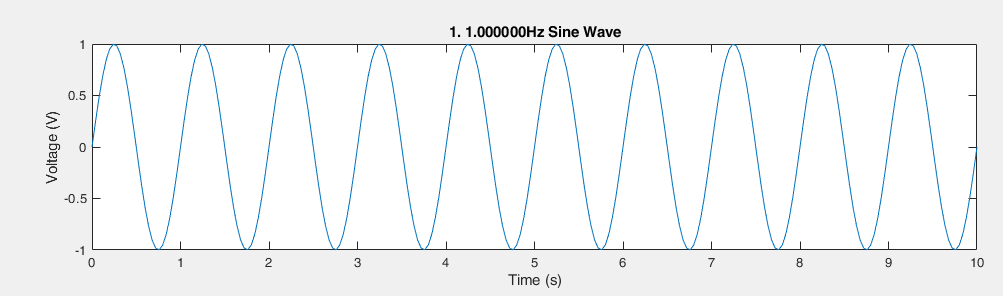
\includegraphics[width=5in]{1}
		\item Samples/sec: 25.1
		\item 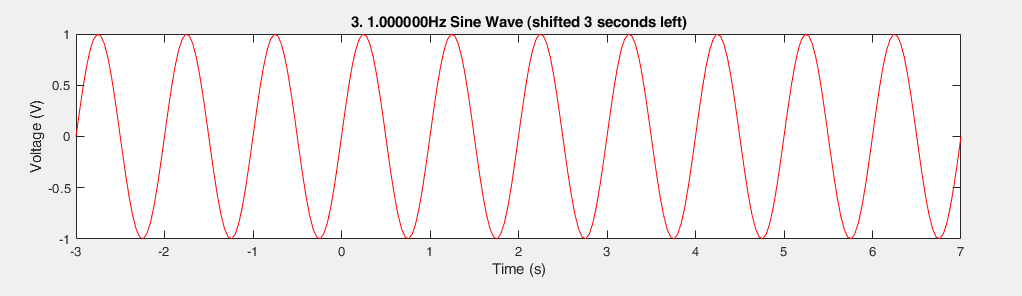
\includegraphics[width=5in]{3}
		\item 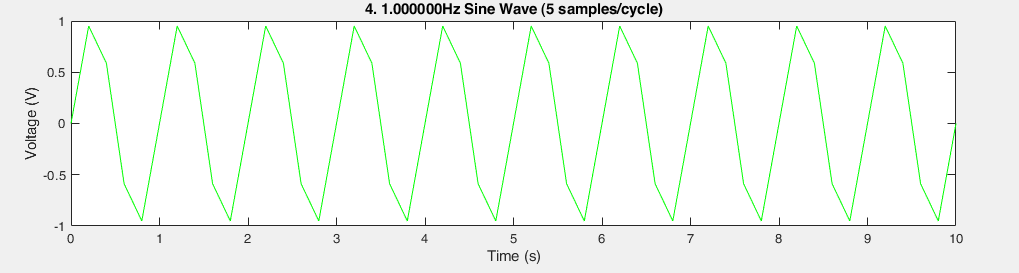
\includegraphics[width=5in]{4}
		\item ~
		
		\begin{tabular}{ccccc}
			0.351660 & 0.830829 & 0.585264 & 0.549724 & 0.917194 \\
			0.285839 & 0.757200 & 0.753729 & 0.380446 & 0.567822 \\
			0.075854 & 0.053950 & 0.530798 & 0.779167 & 0.934011 \\
			0.129906 & 0.568824 & 0.469391 & 0.011902 & 0.337123
		\end{tabular}
	\end{enumerate}

	\lstinputlisting[style=Matlab-editor]{hw1.m}
	
	~\\
	
	\lstinputlisting[style=Matlab-editor]{gen_sine.m}
\end{document}